\documentclass{article}
\usepackage[margin=1in]{geometry}
\usepackage{filecontents}
\usepackage[noadjust]{cite}
\usepackage{listings}
\usepackage{fancyvrb}
\usepackage{tabularx}
\usepackage{adjustbox}
%\usepackage{framed}
\usepackage[listings,skins]{tcolorbox}
\usepackage[skipbelow=\topskip,skipabove=\topskip]{mdframed}
\usepackage{makecell}
\usepackage{tikz}
\usetikzlibrary{matrix,shapes,arrows,positioning}
\mdfsetup{roundcorner=0}

\graphicspath{ {images/} }

\begin{filecontents*}{bibi.bib}
@INBOOK {kubat,
    author    = "Miroslav Kubat",
    title     = "An Introduction to Machine Learning",
    chapter   = "Nearest Neighbor Classifiers",
    publisher = "Springer International",
    year      = "2017",
    edition   = "second"
}
@ONLINE {kurkovsky2011,
    author = "Stan Kurkovsky",
    title  = "Software Engineering: Agile Sofware Development",
    year   = "2011",
    url    = "http://www.cs.ccsu.edu/~stan/classes/cs530/slides11/ch3.pdf"
}
@ONLINE {scikit,
    author = "Scikit-learn",
    title  = "Nearest Neighbors Classification",
    url    = "http://scikit-learn.org/stable/auto_examples/neighbors/plot_classification.html"
}
\end{filecontents*}   

\title{%
       The Effect of Irrelevant Attributes on \textit{\textit{k}}-NN Classifiers}
\author{Lloyd Beaufils, Jerry Bonnell, Gururaj Shriram}
\date{\today}


%{}

\begin{document}
\maketitle

\section{Task}

\textit{\textit{k}}-NN classifiers: Investigate the detrimental effect of irrelevant attributes. Method: create some absolutely clean datafile where you know all attributes are relevant; then, keep adding groups of randomly generated attributes.

\section{Introduction}

The \textit{\textit{k}}-NN classifier is a version of the Nearest Neighbor classifier that looks at \textit{\textit{k}} neighbors as opposed to one. For any given example, the classifier finds its \textit{\textit{k}} nearest neighbors and chooses a class label based upon those of those neighbors. Since this classifier makes use of geometric distances to other examples when deciding class labels, it is essential that those examples be relevant. Each attribute contributes equally to the distance, so attributes that should have no bearing on the class label can quickly overpower the relevant attributes and lead to improper classification. With the irrelevant attributes adding essentially random values to and dominating the distance, the classifier degenerates until it does little better than label classes at random. This behavior is dependent upon the ratio of relevant attributes to irrelevant attributes. The higher that ratio, the less of a negative impact the irrelevant attributes will have. The more irrelevant attributes, then the more terms negatively impacting the distance formula and the worse the classifier will perform, on average. Our group has run some tests to obtain evidence of these claims, and in this paper, we outline our findings.

\section{Method}

For this project, we used two \textit{k}-NN classifiers written in Python to examine our datasets. The first is our own algorithm which was implemented using Table 3.2 in \cite{kubat}. The second is imported from the SciKit-learn, a popular machine learning library that has implemented many of the classifiers present in the textbook \cite{scikit}. This additional check is a cross-check between our "simple" classifier and one implemented by experts, i.e. Scikit-learn. If the classifiers perform similarly, then we expect that our findings are reliable.  \\  

The two algorithms have mostly the same output, but there are slight differences. For the \textit{k}=1 case, the two algorithms are actually identical -- they behave exactly the same way in classifying the data. The differences arise when \textit{k} is greater than one. We determine this difference to be in how we break ties that arise from having more than two possible classes. When determining the class of a piece of data, our implementation sorts class labels based on the number of nearest neighbors within that class. We then randomly choose a class from the subset of classes with the highest frequency of nearest neighbors. This randomness leads to minor differences between the two algorithms. \\

Irrelevant attributes are added in groups of two, with an initial control group of zero irrelevant attributes. To add irrelevant attributes, we used a normal distribution where $\mu$ = 10 and $\sigma$ = 1. The purpose of using this distribution, rather than employing a random number generator, is to create values that mimic irrelevant attributes in realistic domains. Akin to circumstances where engineers do not know which attributes are relevant and which are not, we strive to simulate similar conditions by adding irrelevant attribute values that "act" like any other attribute. The value of $\mu$ and $\sigma$ are gradually increased as groups of irrelevant attributes are added. This resulted in giving the irrelevant attribute values spread without dominating the data due to scaling. Additional research could compare the impact of irrelevant attribute values created by a random number generator and that of the normal distribution that we used.  \\

Finally, we randomly partitioned the datasets into testing and training sets with a ratio of 3:7, respectively. We employed random subsampling to make certain that our training set was representative of the data, and reported the average of all the testing sets. This will ensure that the results are reliable. The division of training and testing set was done 100 times, yielding 100 testing sets. \\   

We ran these classifiers on two separate datasets -- the Iris dataset from the UCI repository and the Animals dataset that we fabricated. Finally, we examined the Wine dataset from the UCI repository to verify that it is the addition of irrelevant, not \textit{relevant}, attributes that lead to poor performance.  The results of our experiments are summarized below.

\section{Iris Dataset}

We obtained the Iris dataset from the UCI machine learning repository. The attributes are sepal and petal length and width, and the examples are classified into one of three species of iris. This domain is well-known for its sheer simplicity, and this simplicity aids us in demonstrating our findings. However, we are keen to note that sepal width is removed from the dataset because of its negative correlation to the data. As required by the task, our goal is to guarantee datasets that are as clean as possible. \\ 

With no irrelevant attributes, the k-NN classifiers (with k ranging from 1 to 9) all classify randomly-partitioned testing sets with at least 95\% accuracy. Our data clearly show that adding irrelevant attributes immediately worsens our accuracy rate, plummeting about twenty points when two irrelevant attributes are added to the dataset. This downward trend continues all the way until the accuracy rate is around an abysmal 30\% with 18 irrelevant attributes. This is the case for both\textit{ k}-NN classifiers, with varied values for \textit{k}. The error rate is over 66\%, indicating that having irrelevant attributes makes the classifier do worse than random. The irrelevant attributes actively misleads the learner's decision-making, thus yielding a classifier that does worse than a class determined by a fair coin flip. The sharpest drop in accuracy occurs with the addition of the first 6 irrelevant attributes. This makes sense because the amount of bad values eclipse and overcome the amount of good values in the distance formula (3 relevant attributes), so at that point it reaches and dips slightly below 40\%, which is slightly better than pure randomness because the relevant attributes contribute slightly to picking the correct class. \\

This shows our classifier with all values of k we tested on the Iris dataset. For all classifiers, the steepest drop in accuracy is with the introduction of the first 6 irrelevant attributes, after which our classifier converges at around 30\% accuracy. \\


\section{Animal Dataset}

The Animal dataset yielded similar results to the Iris dataset. We generated this data programmatically, specifying ranges for valid attributes and generating random numbers within those ranges. There are 5 classes representing different animals, with both relevant (correlated) and irrelevant attributes. The \textit{k}-NN classifiers do a slightly poorer job with no irrelevant attributes when compared to those classifying the Iris dataset. With only relevant attributes, both classifiers average about 91\% accuracy across varying values for \textit{k}. The higher the \textit{k} value, the more accurate the classifier is. Again, as with the Iris dataset, the classifiers decrease in accuracy with the addition of irrelevant attributes. However, for this dataset, the decline is steadier and more gradual. The accuracy rate yields around 25\%, which is slightly lower than the performance on the Iris dataset. However, this makes sense since there are more classes (5 vs 3), so when the classification approaches random selection, there is a lower chance that any specific class is selected.

\section{Wine Dataset}

To verify that the decrease in accuracy is a result of adding irrelevant attributes and not a result of simply adding attributes in general, we performed an additional test on the Wine dataset from the UCI repository. This dataset contains 13 attributes. Our test was as follows. First, we selected only 2 of the 13 attributes and ran our \textit{k}-NN classifier on it. Then, we repeated this process, adding two of the valid attributes at a time until we were using 12 of them. This stands in contrast to our previous tests, as no irrelevant attributes were introduced. What we found was as expected- the accuracy did not decrease as a result of having many attributes. Besides a dip at the ‘6 attribute’ mark (it would appear that one attribute was less relevant than initially believed, or perhaps improperly scaled), the accuracy was either the same or better as a result of having more relevant attributes. This just reinforces the fact that it is the irrelevant attributes that are responsible for the increased error rate in the \textit{k}-NN classifiers.

\section{Conclusion}

After all our experiments, we conclude that irrelevant attributes very clearly increase the error rate of nearest neighbor classifiers. The intuition is straightforward, and our experimental results back it up. The irrelevant attributes add terms to the distance formula that end up obfuscating the result and causing classifiers to deteriorate to randomness. We tested two classifiers on two datasets and found the same results throughout every test. Furthermore, we tested adding only relevant attributes to see if it would have the same effect and it did not. The cause of the decrease in accuracy is the irrelevant attributes, and these tests show just how dangerous they can be. To reduce a classifier from near-perfect accuracy to random performance is a very serious matter, and great care must be taken to ensure that no irrelevant attributes are used when making any classifications with machine learning.

\bibliographystyle{abbrv}
\bibliography{bibi} 

\begin{figure}[hbt]
\centering
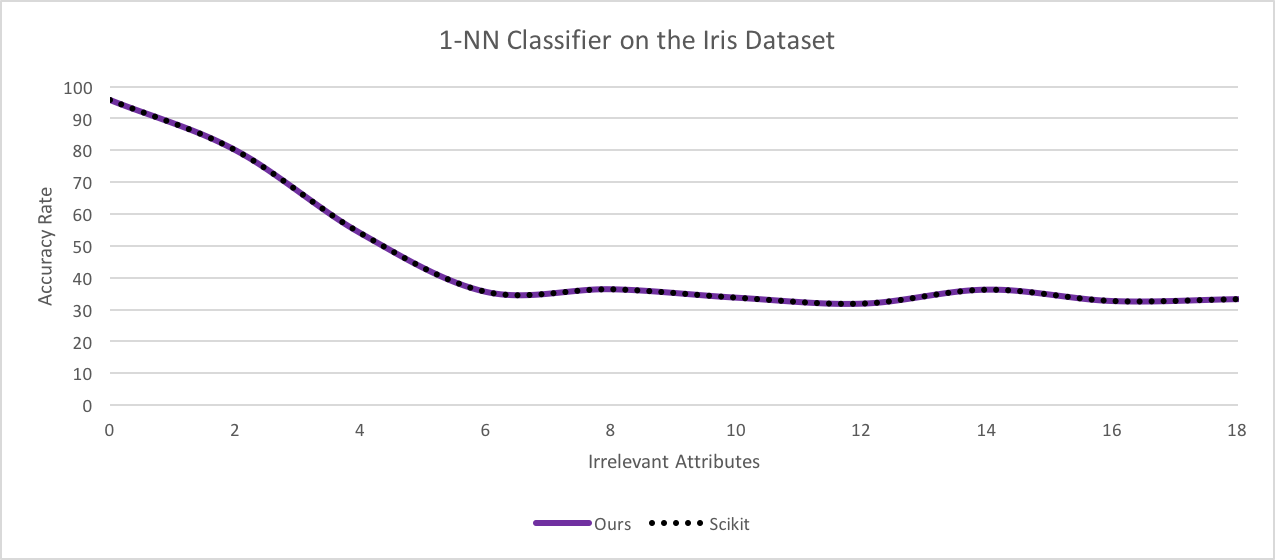
\includegraphics[scale=0.7]{ours-vs-scikit} \\
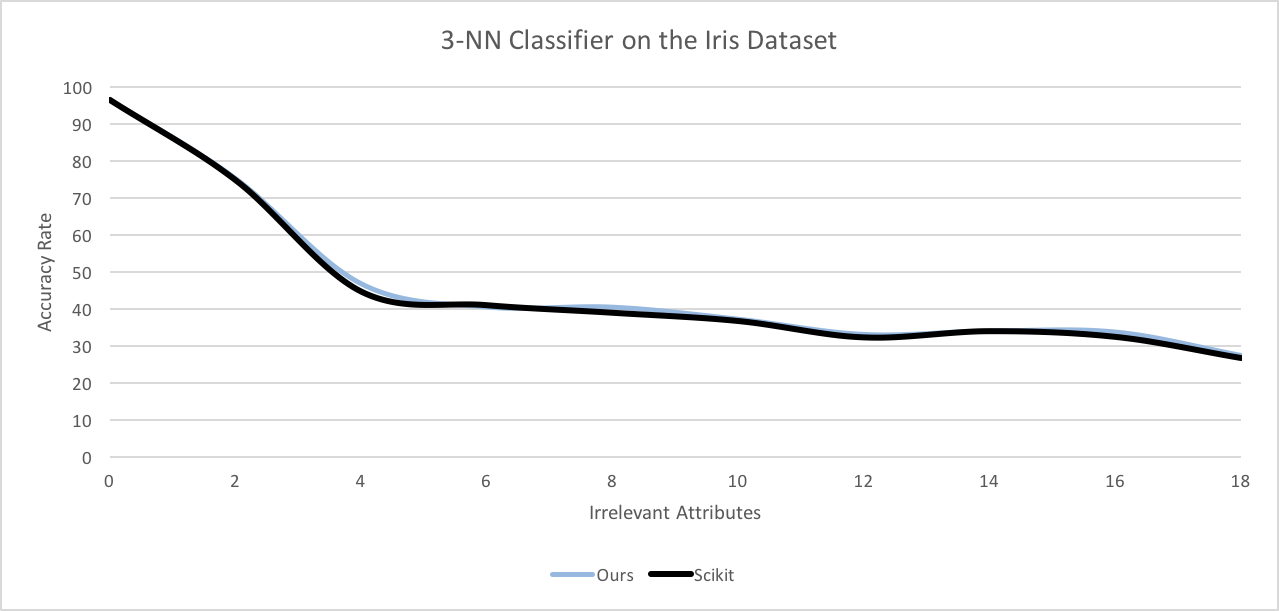
\includegraphics[scale=0.7]{ours-vs-scikit2} 
\caption{These two graphs show the performance of our classifier against the Scikit \textit{k}-NN classifier. They behave identically for \textit{k} = 1 but begin to vary at k-values higher than one.}
\end{figure}

\begin{figure}[hbt]
\centering
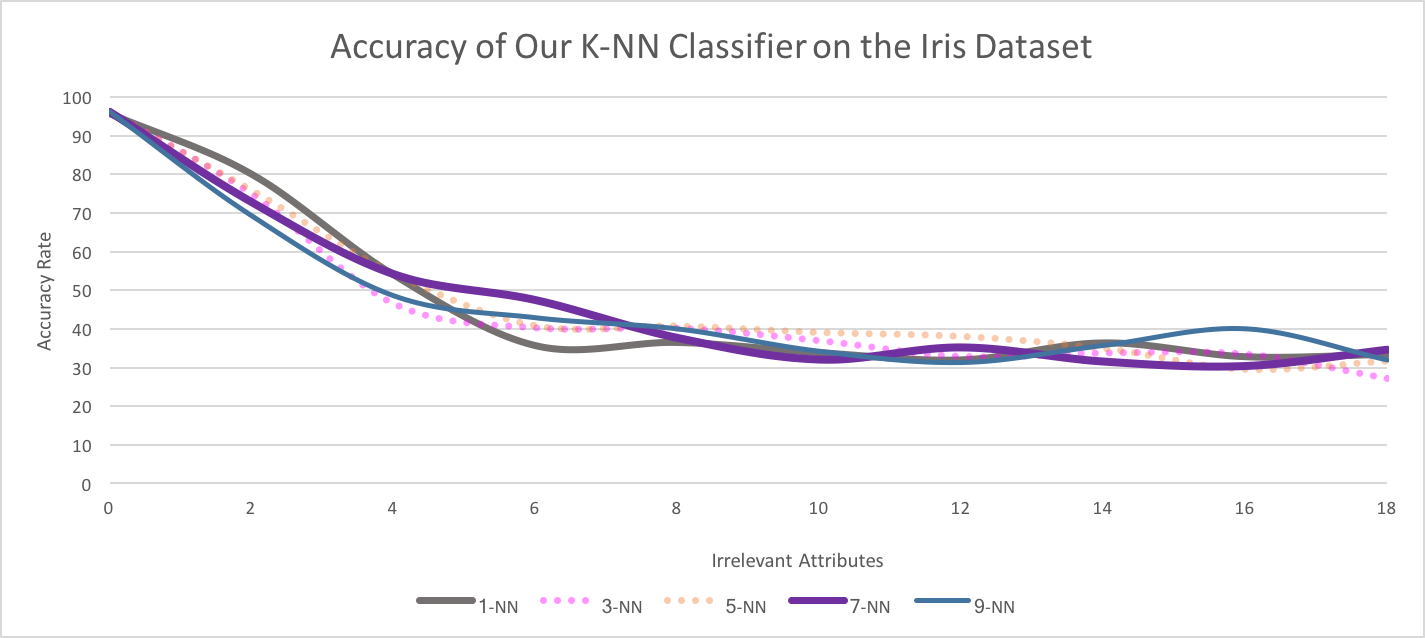
\includegraphics[scale=0.6]{our-knn-iris-full} 
\caption{This shows our classifier with all values of \textit{k} we tested on the Iris dataset. For all classifiers, the steepest drop in accuracy is with the introduction of the first 6 irrelevant attributes, after which our classifier converges at around 30\% accuracy.}
\end{figure}

\begin{figure}[hbt]
\centering
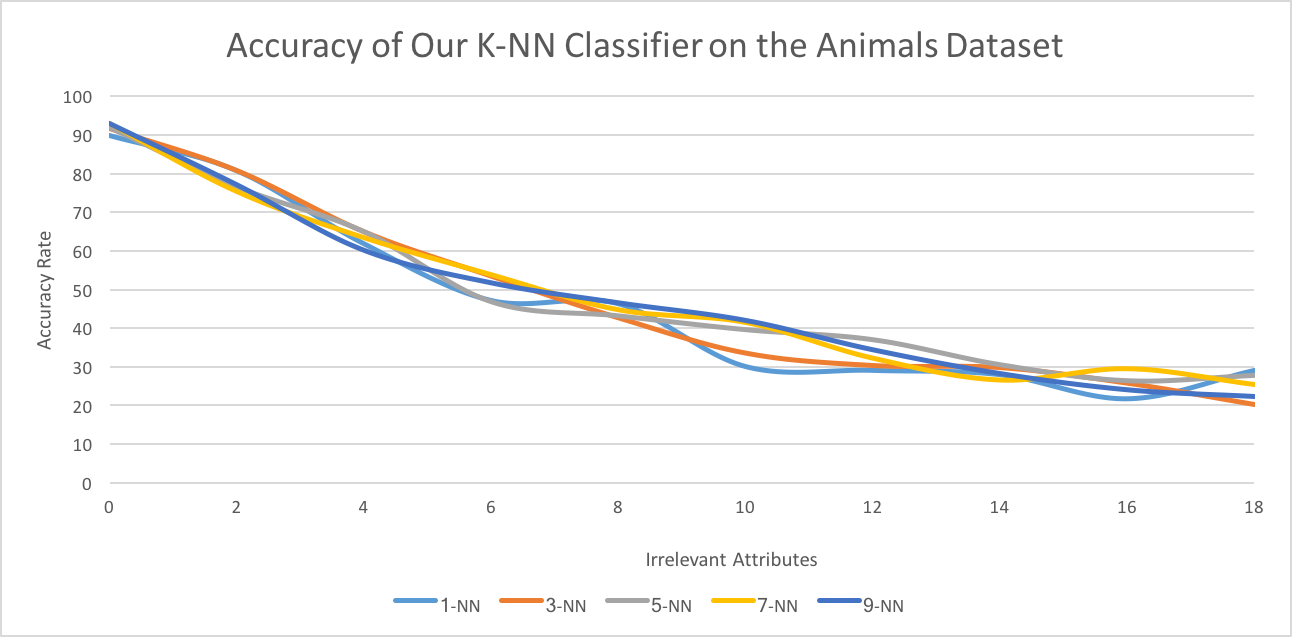
\includegraphics[scale=0.7]{our-knn-animals-full} 
\caption{Irrelevant attributes again are shown to decrease the accuracy rate for all values of \textit{k} in our classifier. Here, the descent is a bit more gradual, but once more the accuracy ends up at around 30\%.}
\end{figure}

\begin{figure}[hbt]
\centering
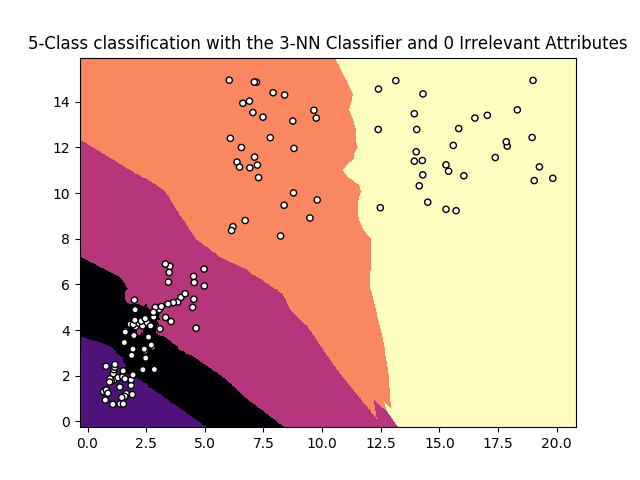
\includegraphics[scale=0.55]{animals-colormap-1} 
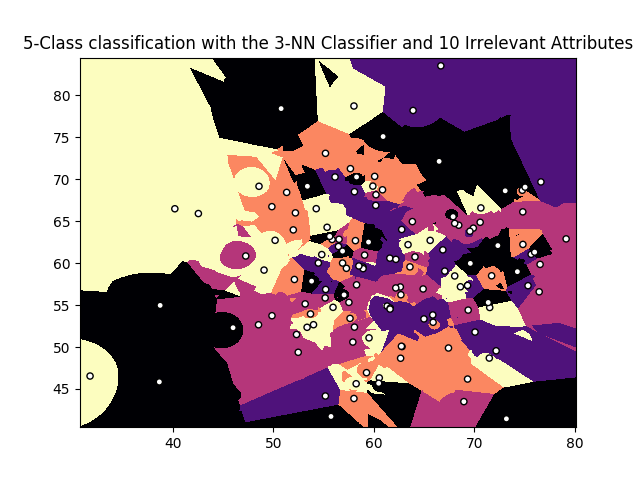
\includegraphics[scale=0.55]{animals-colormap-2}
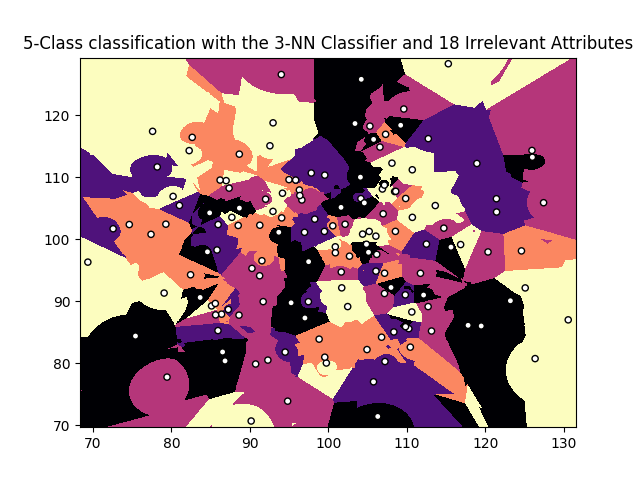
\includegraphics[scale=0.55]{animals-colormap-3}  
\caption{The first color map shows where an example would have to land in the Iris dataset to be classified as one of the three classes. This map uses two relevant attributes on the axes. The latter two color maps show that as the ranges of irrelevant attributes increase, the classification suffers as there is no correlation between an example's classification and the example's irrelevant attribute value.}
\end{figure}

\begin{figure}[hbt]
\centering
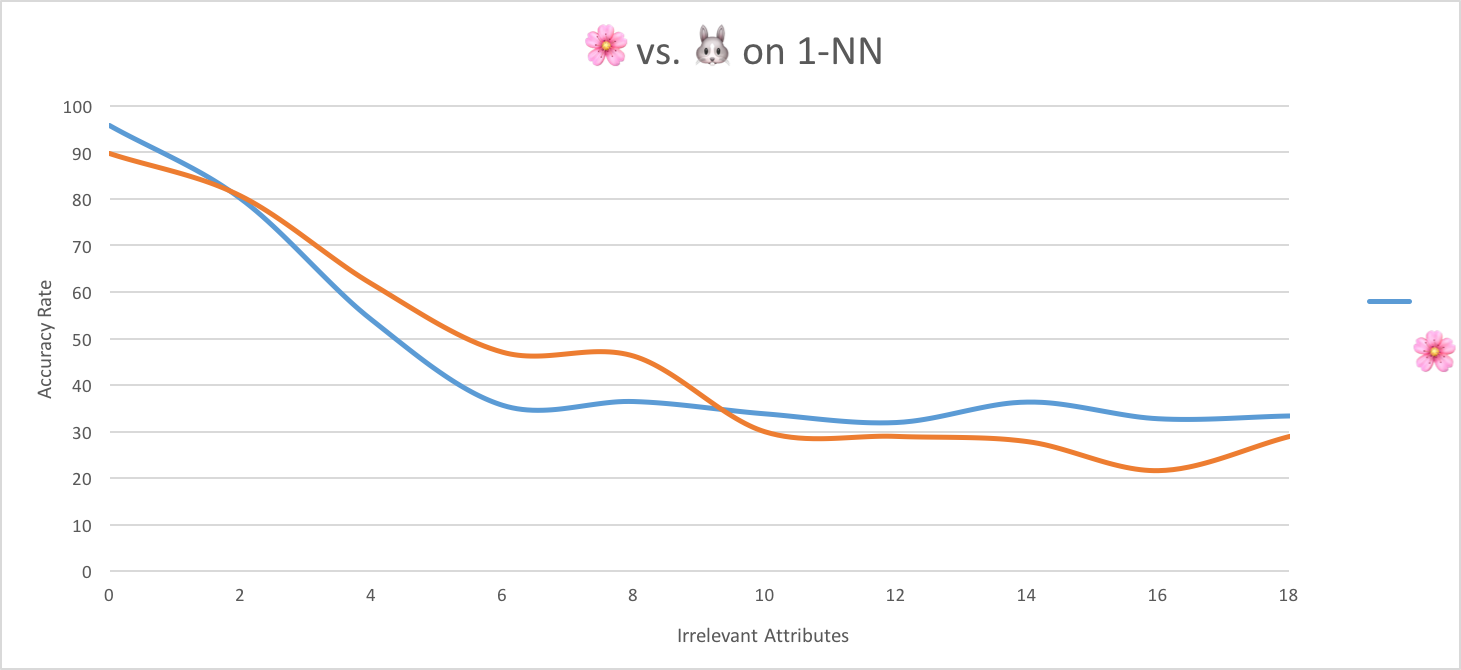
\includegraphics[scale=0.6]{iris-vs-animals} 
\caption{This graph compares the performance of our 1-NN classifier on both datasets. It demonstrates how the irrelevant attributes cause a sharper decline in the Iris dataset and how they decrease the classifier’s accuracy on both datasets.}
\end{figure}

\begin{figure}[hbt]
\centering
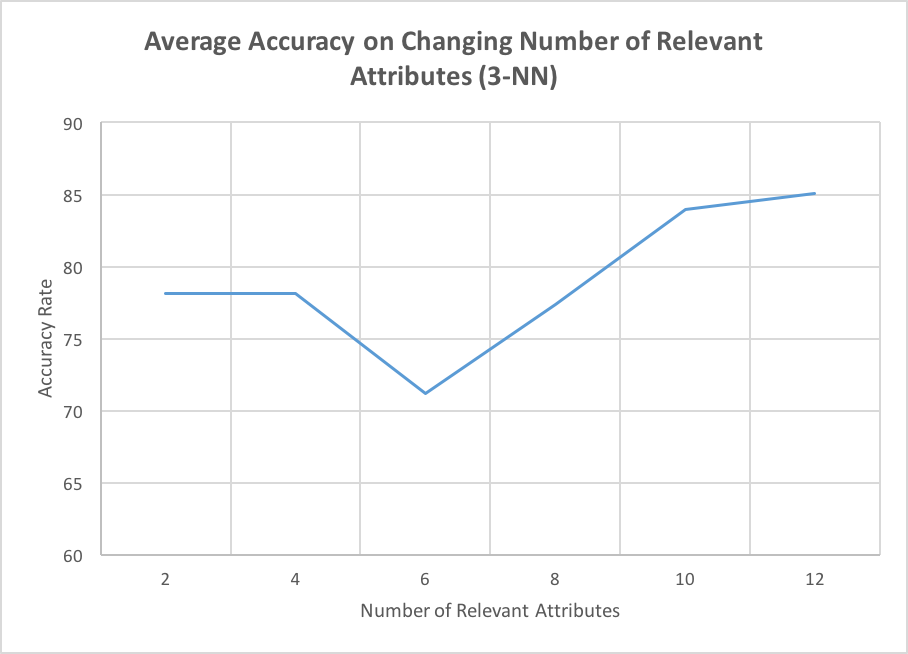
\includegraphics[scale=0.7]{wine-accuracy} 
\caption{This graph shows our 3-NN on the Wine dataset. It demonstrates that the lower accuracy demonstrated in all other graphs is not merely a result of additional attributes, but of specifically irrelevant attributes. Here we add relevant attributes two at a time and the accuracy is improved.}
\end{figure}
\end{document}
